\documentclass{standalone}
\usepackage{tikz}
\usetikzlibrary{patterns, positioning}
\usepackage[sfdefault]{ClearSans} %% option 'sfdefault' activates Clear Sans as the default text font
\usepackage[T1]{fontenc}

\begin{document}
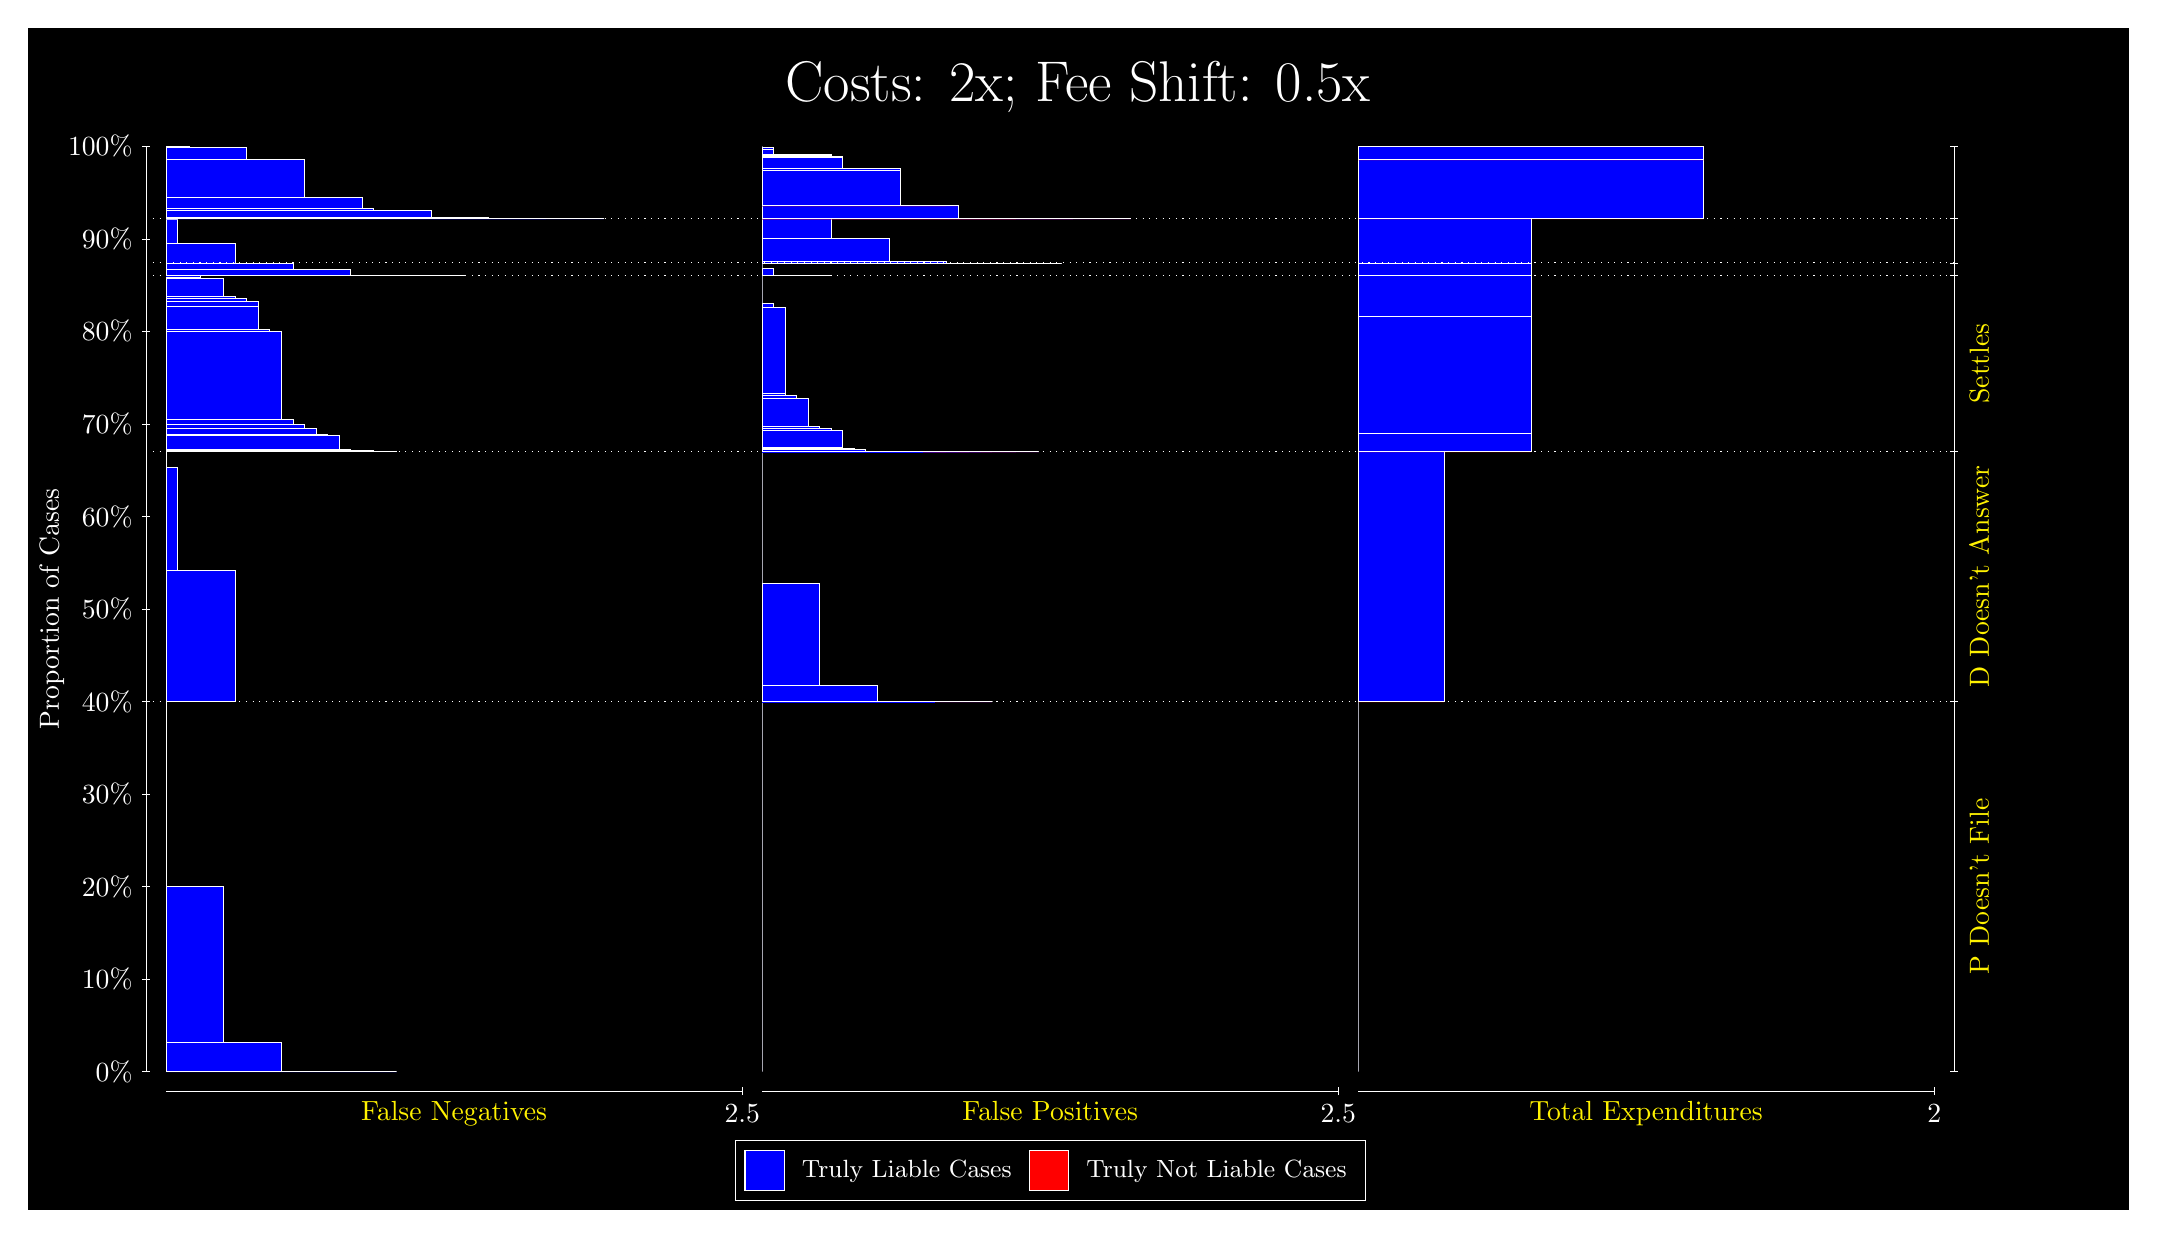
\begin{tikzpicture}
\draw[fill=black] (0,0) rectangle (26.667,15);
\draw[text=white] (0,13.5) rectangle (26.667,15) node[midway] {\huge Costs: 2x; Fee Shift: 0.5x};
\draw[white, very thin] (1.5,1.75) -- (1.5,13.5);
\node[rotate=90, text=white, anchor=center] at (0.3, 7.625) {Proportion of Cases};
\draw[white, very thin] (1.45,1.75) -- (1.55,1.75);
\node[text=white, anchor=east] at (1.45, 1.75) {0\%};
\draw[white, very thin] (1.45,2.925) -- (1.55,2.925);
\node[text=white, anchor=east] at (1.45, 2.925) {10\%};
\draw[white, very thin] (1.45,4.1) -- (1.55,4.1);
\node[text=white, anchor=east] at (1.45, 4.1) {20\%};
\draw[white, very thin] (1.45,5.275) -- (1.55,5.275);
\node[text=white, anchor=east] at (1.45, 5.275) {30\%};
\draw[white, very thin] (1.45,6.45) -- (1.55,6.45);
\node[text=white, anchor=east] at (1.45, 6.45) {40\%};
\draw[white, very thin] (1.45,7.625) -- (1.55,7.625);
\node[text=white, anchor=east] at (1.45, 7.625) {50\%};
\draw[white, very thin] (1.45,8.8) -- (1.55,8.8);
\node[text=white, anchor=east] at (1.45, 8.8) {60\%};
\draw[white, very thin] (1.45,9.975) -- (1.55,9.975);
\node[text=white, anchor=east] at (1.45, 9.975) {70\%};
\draw[white, very thin] (1.45,11.15) -- (1.55,11.15);
\node[text=white, anchor=east] at (1.45, 11.15) {80\%};
\draw[white, very thin] (1.45,12.325) -- (1.55,12.325);
\node[text=white, anchor=east] at (1.45, 12.325) {90\%};
\draw[white, very thin] (1.45,13.5) -- (1.55,13.5);
\node[text=white, anchor=east] at (1.45, 13.5) {100\%};

\draw[white, very thin] (24.457,1.75) -- (24.457,13.5);
\draw[white, very thin] (24.407,1.75) -- (24.507,1.75);
\node[anchor=west] at (24.407, 1.75) {};
\draw[white, very thin] (24.407,6.4489) -- (24.507,6.4489);
\node[anchor=west] at (24.407, 6.4489) {};
\draw[white, very thin] (24.407,9.6236) -- (24.507,9.6236);
\node[anchor=west] at (24.407, 9.6236) {};
\draw[white, very thin] (24.407,11.861) -- (24.507,11.861);
\node[anchor=west] at (24.407, 11.861) {};
\draw[white, very thin] (24.407,12.02) -- (24.507,12.02);
\node[anchor=west] at (24.407, 12.02) {};
\draw[white, very thin] (24.407,12.582) -- (24.507,12.582);
\node[anchor=west] at (24.407, 12.582) {};
\draw[white, very thin] (24.407,13.5) -- (24.507,13.5);
\node[anchor=west] at (24.407, 13.5) {};

\draw[white, very thin, fill=blue] (1.75,1.75) rectangle (4.6775,1.75);
\draw[white, very thin, fill=blue] (1.75,1.75) rectangle (3.9457,1.7532);
\draw[white, very thin, fill=blue] (1.75,1.7532) rectangle (3.2138,2.126);
\draw[white, very thin, fill=blue] (1.75,2.126) rectangle (2.4819,4.1027);
\draw[white, very thin, fill=red] (1.75,4.1027) rectangle (1.75,4.1027);
\draw[white, very thin, fill=blue] (1.75,4.1027) rectangle (1.75,6.4489);
\draw[white, very thin, fill=blue] (1.75,6.4489) rectangle (2.6283,8.1163);
\draw[white, very thin, fill=blue] (1.75,8.1163) rectangle (1.8964,9.4205);
\draw[white, very thin, fill=red] (1.75,9.4205) rectangle (1.75,9.4205);
\draw[white, very thin, fill=blue] (1.75,9.4205) rectangle (1.75,9.6236);
\draw[white, very thin, fill=blue] (1.75,9.6236) rectangle (4.6775,9.631);
\draw[white, very thin, fill=blue] (1.75,9.631) rectangle (4.3848,9.6368);
\draw[white, very thin, fill=blue] (1.75,9.6368) rectangle (4.092,9.6491);
\draw[white, very thin, fill=blue] (1.75,9.6491) rectangle (3.9457,9.8268);
\draw[white, very thin, fill=blue] (1.75,9.8268) rectangle (3.7993,9.8369);
\draw[white, very thin, fill=blue] (1.75,9.8369) rectangle (3.6529,9.9171);
\draw[white, very thin, fill=blue] (1.75,9.9171) rectangle (3.5065,9.9732);
\draw[white, very thin, fill=blue] (1.75,9.9732) rectangle (3.3602,10.034);
\draw[white, very thin, fill=blue] (1.75,10.034) rectangle (3.2138,11.153);
\draw[white, very thin, fill=blue] (1.75,11.153) rectangle (3.0674,11.181);
\draw[white, very thin, fill=blue] (1.75,11.181) rectangle (2.921,11.471);
\draw[white, very thin, fill=blue] (1.75,11.471) rectangle (2.921,11.535);
\draw[white, very thin, fill=blue] (1.75,11.535) rectangle (2.7746,11.57);
\draw[white, very thin, fill=blue] (1.75,11.57) rectangle (2.6283,11.596);
\draw[white, very thin, fill=blue] (1.75,11.596) rectangle (2.4819,11.822);
\draw[white, very thin, fill=blue] (1.75,11.822) rectangle (2.3355,11.829);
\draw[white, very thin, fill=blue] (1.75,11.829) rectangle (2.1891,11.843);
\draw[white, very thin, fill=blue] (1.75,11.843) rectangle (2.1891,11.858);
\draw[white, very thin, fill=blue] (1.75,11.858) rectangle (2.0428,11.859);
\draw[white, very thin, fill=blue] (1.75,11.859) rectangle (1.8964,11.86);
\draw[white, very thin, fill=red] (1.75,11.86) rectangle (1.75,11.86);
\draw[white, very thin, fill=blue] (1.75,11.86) rectangle (1.75,11.861);
\draw[white, very thin, fill=blue] (1.75,11.861) rectangle (5.5558,11.861);
\draw[white, very thin, fill=blue] (1.75,11.861) rectangle (4.8239,11.866);
\draw[white, very thin, fill=blue] (1.75,11.866) rectangle (4.092,11.933);
\draw[white, very thin, fill=blue] (1.75,11.933) rectangle (3.3602,12.018);
\draw[white, very thin, fill=blue] (1.75,12.018) rectangle (2.6283,12.02);
\draw[white, very thin, fill=red] (1.75,12.02) rectangle (1.75,12.02);
\draw[white, very thin, fill=blue] (1.75,12.02) rectangle (2.6283,12.271);
\draw[white, very thin, fill=blue] (1.75,12.271) rectangle (1.8964,12.568);
\draw[white, very thin, fill=red] (1.75,12.568) rectangle (1.75,12.568);
\draw[white, very thin, fill=blue] (1.75,12.568) rectangle (1.75,12.582);
\draw[white, very thin, fill=blue] (1.75,12.582) rectangle (7.3123,12.582);
\draw[white, very thin, fill=blue] (1.75,12.582) rectangle (6.5805,12.582);
\draw[white, very thin, fill=blue] (1.75,12.582) rectangle (5.8486,12.599);
\draw[white, very thin, fill=blue] (1.75,12.599) rectangle (5.7022,12.599);
\draw[white, very thin, fill=blue] (1.75,12.599) rectangle (5.1167,12.685);
\draw[white, very thin, fill=blue] (1.75,12.685) rectangle (4.9703,12.689);
\draw[white, very thin, fill=blue] (1.75,12.689) rectangle (4.3848,12.709);
\draw[white, very thin, fill=blue] (1.75,12.709) rectangle (4.2384,12.855);
\draw[white, very thin, fill=blue] (1.75,12.855) rectangle (3.6529,12.855);
\draw[white, very thin, fill=blue] (1.75,12.855) rectangle (3.5065,13.336);
\draw[white, very thin, fill=blue] (1.75,13.336) rectangle (2.921,13.336);
\draw[white, very thin, fill=blue] (1.75,13.336) rectangle (2.7746,13.492);
\draw[white, very thin, fill=blue] (1.75,13.492) rectangle (2.0428,13.5);
\draw[white, very thin, fill=red] (1.75,13.5) rectangle (1.75,13.5);
\draw[white, very thin, fill=blue] (1.75,13.5) rectangle (1.75,13.5);
\draw[white, very thin, fill=red] (9.3189,1.75) rectangle (9.3189,1.75);
\draw[white, very thin, fill=blue] (9.3189,1.75) rectangle (9.3189,6.4489);
\draw[white, very thin, fill=red] (9.3189,6.4489) rectangle (12.246,6.4489);
\draw[white, very thin, fill=blue] (9.3189,6.4489) rectangle (12.246,6.4489);
\draw[white, very thin, fill=blue] (9.3189,6.4489) rectangle (11.515,6.4493);
\draw[white, very thin, fill=blue] (9.3189,6.4493) rectangle (10.783,6.652);
\draw[white, very thin, fill=blue] (9.3189,6.652) rectangle (10.051,7.9563);
\draw[white, very thin, fill=blue] (9.3189,7.9563) rectangle (9.3189,9.6236);
\draw[white, very thin, fill=red] (9.3189,9.6236) rectangle (12.832,9.6236);
\draw[white, very thin, fill=blue] (9.3189,9.6236) rectangle (12.832,9.6236);
\draw[white, very thin, fill=red] (9.3189,9.6236) rectangle (12.539,9.6236);
\draw[white, very thin, fill=blue] (9.3189,9.6236) rectangle (12.539,9.6236);
\draw[white, very thin, fill=red] (9.3189,9.6236) rectangle (12.246,9.6236);
\draw[white, very thin, fill=blue] (9.3189,9.6236) rectangle (12.246,9.6236);
\draw[white, very thin, fill=blue] (9.3189,9.6236) rectangle (12.1,9.6236);
\draw[white, very thin, fill=red] (9.3189,9.6236) rectangle (11.954,9.6236);
\draw[white, very thin, fill=blue] (9.3189,9.6236) rectangle (11.954,9.6236);
\draw[white, very thin, fill=blue] (9.3189,9.6236) rectangle (11.807,9.6236);
\draw[white, very thin, fill=red] (9.3189,9.6236) rectangle (11.661,9.6236);
\draw[white, very thin, fill=blue] (9.3189,9.6236) rectangle (11.661,9.6236);
\draw[white, very thin, fill=blue] (9.3189,9.6236) rectangle (11.515,9.6236);
\draw[white, very thin, fill=red] (9.3189,9.6236) rectangle (11.368,9.6236);
\draw[white, very thin, fill=blue] (9.3189,9.6236) rectangle (11.368,9.624);
\draw[white, very thin, fill=blue] (9.3189,9.624) rectangle (11.222,9.624);
\draw[white, very thin, fill=blue] (9.3189,9.624) rectangle (11.075,9.6245);
\draw[white, very thin, fill=red] (9.3189,9.6245) rectangle (11.075,9.6245);
\draw[white, very thin, fill=blue] (9.3189,9.6245) rectangle (11.075,9.625);
\draw[white, very thin, fill=blue] (9.3189,9.625) rectangle (10.929,9.6252);
\draw[white, very thin, fill=blue] (9.3189,9.6252) rectangle (10.783,9.6264);
\draw[white, very thin, fill=blue] (9.3189,9.6264) rectangle (10.636,9.6552);
\draw[white, very thin, fill=blue] (9.3189,9.6552) rectangle (10.49,9.6622);
\draw[white, very thin, fill=blue] (9.3189,9.6622) rectangle (10.344,9.6791);
\draw[white, very thin, fill=blue] (9.3189,9.6791) rectangle (10.344,9.8887);
\draw[white, very thin, fill=blue] (9.3189,9.8887) rectangle (10.197,9.9144);
\draw[white, very thin, fill=blue] (9.3189,9.9144) rectangle (10.051,9.9498);
\draw[white, very thin, fill=blue] (9.3189,9.9498) rectangle (9.9044,10.303);
\draw[white, very thin, fill=blue] (9.3189,10.303) rectangle (9.758,10.332);
\draw[white, very thin, fill=blue] (9.3189,10.332) rectangle (9.6116,10.361);
\draw[white, very thin, fill=blue] (9.3189,10.361) rectangle (9.6116,11.451);
\draw[white, very thin, fill=blue] (9.3189,11.451) rectangle (9.4652,11.511);
\draw[white, very thin, fill=blue] (9.3189,11.511) rectangle (9.3189,11.861);
\draw[white, very thin, fill=red] (9.3189,11.861) rectangle (10.197,11.861);
\draw[white, very thin, fill=blue] (9.3189,11.861) rectangle (10.197,11.863);
\draw[white, very thin, fill=blue] (9.3189,11.863) rectangle (9.4652,11.948);
\draw[white, very thin, fill=blue] (9.3189,11.948) rectangle (9.3189,12.02);
\draw[white, very thin, fill=red] (9.3189,12.02) rectangle (13.125,12.02);
\draw[white, very thin, fill=blue] (9.3189,12.02) rectangle (13.125,12.02);
\draw[white, very thin, fill=blue] (9.3189,12.02) rectangle (12.393,12.02);
\draw[white, very thin, fill=blue] (9.3189,12.02) rectangle (11.661,12.034);
\draw[white, very thin, fill=blue] (9.3189,12.034) rectangle (10.929,12.331);
\draw[white, very thin, fill=blue] (9.3189,12.331) rectangle (10.197,12.582);
\draw[white, very thin, fill=red] (9.3189,12.582) rectangle (14.003,12.582);
\draw[white, very thin, fill=blue] (9.3189,12.582) rectangle (14.003,12.582);
\draw[white, very thin, fill=red] (9.3189,12.582) rectangle (13.271,12.582);
\draw[white, very thin, fill=blue] (9.3189,12.582) rectangle (13.271,12.582);
\draw[white, very thin, fill=red] (9.3189,12.582) rectangle (12.539,12.582);
\draw[white, very thin, fill=blue] (9.3189,12.582) rectangle (12.539,12.59);
\draw[white, very thin, fill=blue] (9.3189,12.59) rectangle (11.807,12.746);
\draw[white, very thin, fill=red] (9.3189,12.746) rectangle (11.807,12.746);
\draw[white, very thin, fill=blue] (9.3189,12.746) rectangle (11.807,12.746);
\draw[white, very thin, fill=red] (9.3189,12.746) rectangle (11.661,12.746);
\draw[white, very thin, fill=blue] (9.3189,12.746) rectangle (11.661,12.746);
\draw[white, very thin, fill=blue] (9.3189,12.746) rectangle (11.075,13.195);
\draw[white, very thin, fill=blue] (9.3189,13.195) rectangle (11.075,13.227);
\draw[white, very thin, fill=red] (9.3189,13.227) rectangle (10.929,13.227);
\draw[white, very thin, fill=blue] (9.3189,13.227) rectangle (10.929,13.227);
\draw[white, very thin, fill=blue] (9.3189,13.227) rectangle (10.344,13.36);
\draw[white, very thin, fill=blue] (9.3189,13.36) rectangle (10.344,13.373);
\draw[white, very thin, fill=blue] (9.3189,13.373) rectangle (10.197,13.392);
\draw[white, very thin, fill=red] (9.3189,13.392) rectangle (10.197,13.392);
\draw[white, very thin, fill=blue] (9.3189,13.392) rectangle (10.197,13.393);
\draw[white, very thin, fill=blue] (9.3189,13.393) rectangle (9.6116,13.397);
\draw[white, very thin, fill=blue] (9.3189,13.397) rectangle (9.6116,13.397);
\draw[white, very thin, fill=blue] (9.3189,13.397) rectangle (9.4652,13.467);
\draw[white, very thin, fill=blue] (9.3189,13.467) rectangle (9.4652,13.483);
\draw[white, very thin, fill=blue] (9.3189,13.483) rectangle (9.3189,13.5);
\draw[white, very thin, fill=red] (16.888,1.75) rectangle (16.888,1.75);
\draw[white, very thin, fill=blue] (16.888,1.75) rectangle (16.888,6.4489);
\draw[white, very thin, fill=red] (16.888,6.4489) rectangle (17.986,6.4489);
\draw[white, very thin, fill=blue] (16.888,6.4489) rectangle (17.986,9.6236);
\draw[white, very thin, fill=red] (16.888,9.6236) rectangle (19.083,9.6236);
\draw[white, very thin, fill=blue] (16.888,9.6236) rectangle (19.083,9.8615);
\draw[white, very thin, fill=red] (16.888,9.8615) rectangle (19.083,9.8615);
\draw[white, very thin, fill=blue] (16.888,9.8615) rectangle (19.083,11.346);
\draw[white, very thin, fill=red] (16.888,11.346) rectangle (19.083,11.346);
\draw[white, very thin, fill=blue] (16.888,11.346) rectangle (19.083,11.861);
\draw[white, very thin, fill=red] (16.888,11.861) rectangle (19.083,11.861);
\draw[white, very thin, fill=blue] (16.888,11.861) rectangle (19.083,12.02);
\draw[white, very thin, fill=red] (16.888,12.02) rectangle (19.083,12.02);
\draw[white, very thin, fill=blue] (16.888,12.02) rectangle (19.083,12.582);
\draw[white, very thin, fill=red] (16.888,12.582) rectangle (21.279,12.582);
\draw[white, very thin, fill=blue] (16.888,12.582) rectangle (21.279,13.33);
\draw[white, very thin, fill=red] (16.888,13.33) rectangle (21.279,13.33);
\draw[white, very thin, fill=blue] (16.888,13.33) rectangle (21.279,13.5);
\draw[white, dotted] (1.5,6.4489) -- (24.457,6.4489);
\draw[white, dotted] (1.5,9.6236) -- (24.457,9.6236);
\draw[white, dotted] (1.5,11.861) -- (24.457,11.861);
\draw[white, dotted] (1.5,12.02) -- (24.457,12.02);
\draw[white, dotted] (1.5,12.582) -- (24.457,12.582);
\draw[white, very thin] (1.75,1.5) -- (9.0689,1.5);
\node[text=yellow, anchor=north] at (5.4094, 1.5) {False Negatives};
\draw[white, very thin] (9.0689,1.45) -- (9.0689,1.55);
\node[text=white, anchor=north] at (9.0689, 1.45) {2.5};

\draw[white, very thin] (9.3189,1.5) -- (16.638,1.5);
\node[text=yellow, anchor=north] at (12.978, 1.5) {False Positives};
\draw[white, very thin] (16.638,1.45) -- (16.638,1.55);
\node[text=white, anchor=north] at (16.638, 1.45) {2.5};

\draw[white, very thin] (16.888,1.5) -- (24.207,1.5);
\node[text=yellow, anchor=north] at (20.547, 1.5) {Total Expenditures};
\draw[white, very thin] (24.207,1.45) -- (24.207,1.55);
\node[text=white, anchor=north] at (24.207, 1.45) {2};

\node[text=yellow, centered, rotate=90] at (24.777, 4.0995) {P Doesn't File};
\node[text=yellow, centered, rotate=90] at (24.777, 8.0363) {D Doesn't Answer};
\node[text=yellow, centered, rotate=90] at (24.777, 10.742) {Settles};




\draw (12.978300999999998,1.5) node[draw=none] (baseCoordinate) {};
\begin{scope}[align=center]
        \matrix[scale=0.5, draw=white, below=0.5cm of baseCoordinate, nodes={draw}, column sep=0.1cm]{
            \node[rectangle, draw, minimum width=0.5cm, minimum height=0.5cm, fill=blue] {}; &
            \node[draw=none, font=\small, text=white] (B) {Truly Liable Cases}; &
            \node[rectangle, draw, minimum width=0.5cm, minimum height=0.5cm, fill=red] {}; &
            \node[draw=none, font=\small, text=white] (B) {Truly Not Liable Cases}; \\
            };
\end{scope}

\end{tikzpicture}
\end{document}